\documentclass[a4paper,11pt]{article}
\usepackage{pdflscape}
\usepackage[utf8]{inputenc}
\usepackage[T1]{fontenc}
%\usepackage{fourier} % math & rm
%\usepackage{amsthm,amsfonts,amsmath,amssymb,textcomp}
\usepackage{pst-all,pstricks-add,pst-eucl}
\everymath{\displaystyle}
\usepackage{fp,ifthen}
%\usepackage{color}
%\usepackage{graphicx}
\usepackage{setspace}
\usepackage{array}
\usepackage{tabularx}
\usepackage{supertabular}
\usepackage{hhline}
\usepackage{variations}
\usepackage{enumerate}
\usepackage{pifont}
\usepackage{framed}
\usepackage[fleqn]{amsmath}
\usepackage{amssymb}
\usepackage[framed]{ntheorem}
\usepackage{multicol}
\usepackage{kpfonts}
\usepackage{manfnt}

%\usepackage[hmargin=2.5cm, vmargin=2.5cm]{geometry}
\usepackage{vmargin}          % Pour fixer les marges du document
\setmarginsrb
{1.5cm} 	%marge gauche
{0.5cm} 	  %marge en haut
{1.5cm}     %marge droite
{0.5cm}   %marge en bas
{1cm} 	%hauteur de l'entête
{0.5cm}   %distance entre l'entête et le texte
{1cm} 	  %hauteur du pied de page
{0.5cm}     %distance entre le texte et le pied de page

\newcommand{\R}{\mathbb{R}}
\newcommand{\N}{\mathbb{N}}
%\newcommand{\D}{\mathbb{D}}
\newcommand{\Z}{\mathbb{Z}}
\newcommand{\Q}{\mathbb{Q}}
\newcommand{\C}{\mathbb{C}}
\newcommand{\e}{\text{e}}
\newcommand{\dx}{\text{d}x}
\newcommand{\vect}[1]{\mathchoice%
  {\overrightarrow{\displaystyle\mathstrut#1\,\,}}%
  {\overrightarrow{\textstyle\mathstrut#1\,\,}}%
  {\overrightarrow{\scriptstyle\mathstrut#1\,\,}}%
  {\overrightarrow{\scriptscriptstyle\mathstrut#1\,\,}}}
\newcommand\arraybslash{\let\\\@arraycr}
\renewcommand{\theenumi}{\textbf{\arabic{enumi}}}
\renewcommand{\labelenumi}{\textbf{\theenumi.}}
\renewcommand{\theenumii}{\textbf{\alph{enumii}}}
\renewcommand{\labelenumii}{\textbf{\theenumii.}}
\renewcommand{\and}{\wedge}

\theoremstyle{break}
\theorembodyfont{\upshape}
\newframedtheorem{theorem}{Théorème}
\newframedtheorem{proposition}{Proposition}
\newframedtheorem{definition}{Définition}

\newtheorem{Term}{Terminologie}
\newtheorem{Rq}{Remarque}
\newtheorem{exemple}{Exemple}
%\newtheorem{exo}{Exercice}

%\theorembodyfont{\small \sffamily}
%\newtheorem{sol}{solution}

\newenvironment{sol}% 
{\def\FrameCommand{\hspace{0.5cm} {\color{black} \vrule width 1pt} \hspace{-0.7cm}}%
  \framed {\advance\hsize-\width}
  \noindent \small \sffamily  %\underline{Solution :}%\\
}%
{\endframed}

\newrgbcolor{vert}{0 0.4 0}
\newrgbcolor{bistre}{1 .50 .30}
\setlength\tabcolsep{1mm}
\renewcommand\arraystretch{1.3}

\everymath{\displaystyle}
\hyphenpenalty 10000 %supprime toutes les césures
%\setcounter{secnumdepth}{0}
%\newcounter{saveenum}

\usepackage[frenchb]{babel}
%\usepackage{fancyhdr,lastpage}
%\usepackage{fancybox}

%\headheight 15.0 pt
%\fancyhead[L]{Leçon}
%\fancyhead[C]{}
%\fancyhead[R]{Chapitre 1}
%\fancyfoot[L]{{\scriptsize\textsl{Thomas Gire Cité scolaire de Lorgues}}}
%\fancyfoot[C]{\scriptsize\thepage}
%\fancyfoot[C]{\scriptsize\thepage/\pageref{LastPage}}

\title{Second Degré.}
\author{}
\date{}

%\pagestyle{empty}
%\pagestyle{fancy}
\usepackage[np]{numprint}

\renewcommand\arraystretch{1.8}

\newcounter{numero}
\newcommand{\exo}{
  \addtocounter{numero}{1}%
  \textbf{\underline{Exercice \arabic{numero}:}}\quad}

\frenchbsetup{StandardEnumerateEnv=true}
\usepackage{etex}
\usepackage{tikz,tkz-tab}
\usepackage{graphicx}
\graphicspath{ {../images/} }





\begin{document}
  %\setlength{\unitlength}{1mm}
  %\setlength\parindent{0mm}
 
  \maketitle


  
  \section{Fonctions polynômes de degré 2.}
  
  
  \begin{definition}
    \begin{itemize}
     \item Une \textbf{fonction polynôme de degré 2} est une fonction $f$ définie sur $\mathbb{R}$
    qui peut être mise sous la forme $f(x)=ax^2+bx+c$ où $a,b,c$ sont trois nombres 
    rééls avec $a$ non nul.
     
     \item L'expression $ax^2+bx+c$ est la \textbf{forme développée} de $f(x)$.
     \item Une fonction polynôme de degré $2$ est aussi appelée 
     \textbf{trinôme} (du second degré).
     \item On appelle \textbf{parabole} la représentation graphique 
     d'un trinôme.
   \end{itemize}    
  \end{definition}
  
  
  
  \begin{exemple}
    Les fonctions suivantes sont-elles des trinômes ?
    \begin{enumerate}
     \item $g(x)=2x^2+3x+1$. 
     \item $h(x)=3(x-1)^2+1$.
     \item $i(x)=4(x-1)(x+2)$.
     \item $i(x)=5x+3$.
     \item $j(x)=x^3+4x^2+1$.
     \end{enumerate}
 
 \end{exemple}
  
  \begin{theorem}[Variations d'un trinôme du second degré]

    Un trinôme $f(x)=ax^2+bx+c$ admet pour variations:
    \begin{itemize}
      \item Si $a>0$
      \[
      \begin{tikzpicture}
	\tkzTabInit{$x$ /1,$f(x)$/2}{$-\infty$, $\alpha$, $+\infty$}
	
	\tkzTabVar{+/$+\infty$,-/$\beta$,+/$+\infty$}
      \end{tikzpicture}
      \] 
      
      \item Si $a<0$
      \[
      \begin{tikzpicture}
	\tkzTabInit{$x$/1,$f(x)$/2}{$-\infty$, $\alpha$, $+\infty$}
	
	\tkzTabVar{-/$-\infty$,+/$\beta$,-/$-\infty$}
      \end{tikzpicture}
      \]
    \end{itemize}
    
    On peut calculer les coordonnées $(\alpha,\beta)$ du sommet $S$ de la 
    parabole grâce aux formules $$\alpha=-\frac{b}{2a} \hspace{1cm} \beta=f(\alpha)$$
    
    De plus, $f$ s'écrit $f(x)=a(x-\alpha)^2+\beta$. Cette écriture est la
    \textbf{forme canonique} du trinôme.
    
    \end{theorem}
    
 %     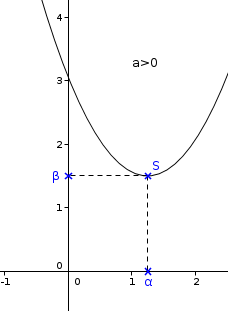
\includegraphics{variationsapos}
 %     \hspace{1cm}
 %     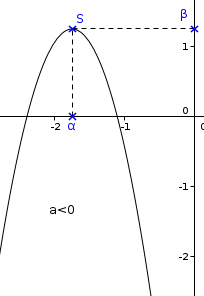
\includegraphics{variationsaneg}
    
 \begin{exemple}
   Pour chacun des trinômes $P(x) = 2x^2+4x-3$ et $Q(x)=-(x-2)^2$ : 
   \begin{enumerate}
    \item Identifier les coefficients $a,b,c$.
    \item Dresser le tableau de variation.
   \end{enumerate}

  
  
 \end{exemple}


     
     \section{Racines et factorisation.}
    
  %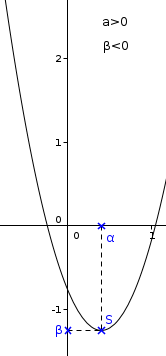
\includegraphics[width=4cm]{aposbetaneg}\hspace{0.3cm}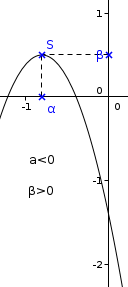
\includegraphics[width=4cm]{anegbetapos}
  
  \begin{definition}
    Soit $f(x)=ax^2+bx+c$ un trinôme du second degré et $\mathcal{P}$ sa représentation 
    graphique.
    
    On appelle \textbf{racines} de $f$ les solutions de l'équation $f(x)=0$. Ce sont les 
    abscisses des points d'intersection entre $\mathcal{P}$ et l'axe des abscisses.
    
  \end{definition}
  
  \begin{exemple}
    Les fonctions suivantes admettent-elles des racines ? Si oui, combien ? 
    Et quelles sont-elles ?
    \begin{enumerate}
     \item $f(x)=3(x+1)(x-2)$. 
     \item $g(x)=2(x-3)^2$.
    \end{enumerate}
  \end{exemple}
  
  \begin{proposition}
   Soit $f(x)$ un trinôme du second degré et $\mathcal{P}$ sa représentation graphique.
    Trois cas peuvent se produire:
   
   \begin{itemize}
    \item $f$ admet $2$ racines, c'est-à-dire $\mathcal{P}$ coupe l'axe des abscisses 
    en $2$ points.
    \item $f$ admet une racine, c'est-à-dire $\mathcal{P}$ est tangente à l'axe
    des abscisses ($1$ point d'intersection).
    
    Dans ce cas, on dit que la racine est une racine double.
    
    \item $f$ n'admet pas de racine, c'est-à-dire $\mathcal{P}$ ne coupe pas l'axe des abscisses.
   \end{itemize}
   
  \end{proposition}
  
  \vspace{10cm}
  
  
  
  \begin{definition}[Discriminant]
    Soit $f(x)$ un trinôme du second degré dont la forme développée réduite
    est $f(x)=ax^2+bx+c$. On appelle \textbf{discriminant} de ce trinôme
    le nombre $\Delta=b^2-4ac$.
    
    
  \end{definition}
  
  \begin{exemple}
    
    Calculer les discriminants des trinômes suivants:
    \begin{enumerate}
     \item Soit $h(x)=x^2-4x+3$.
     \item Soit $i(x)=2x^2-4x+2$.
     \item Soit $j(x)=-3x^2+12x-15$
    \end{enumerate}
   \end{exemple}
  
  \begin{theorem}[Central]
    Soit $f(x)=ax^2+bx+c$ un trinôme.
    \begin{itemize}
     \item  si le discriminant $\Delta$ de $f(x)$ est strictement positif alors
     $f(x)$ admet deux racines :
     $$x_1=\frac{-b-\sqrt{\Delta}}{2a} \hspace{2cm} x_2=\frac{-b+\sqrt{\Delta}}{2a}$$
     
     et on peut factoriser $f(x)$ en $f(x)=a(x-x_1)(x-x_2)$.
     
     \item si le discriminant de $f(x)$ est nul alors $f(x)$ admet une racine double
     $$x_0=-\frac{b}{2a}(=\alpha)$$
     
     et on peut factoriser $f(x)$ en $f(x)=a(x-x_0)^2$.
     
     \item si le discriminant de $f(x)$ est strictement négatif alors
     $f(x)$ ne possède pas de racine.
     
     et on ne peut pas factoriser $f(x)$ en un produit de termes de degré 1.
    \end{itemize}    
  \end{theorem}
  
  \begin{exemple}
    Calculer les racines (éventuelles) des trinômes de l'exemple 4, puis factoriser
    ces trinômes (si possible).
   \end{exemple}
   
\end{document}

On admet que  l'on peut calculer $\beta$ à l'aide la formule $\beta=-\frac{\Delta}{4a}$.

\begin{proposition}[Positions de paraboles]
    Il n'y a que deux possibilités pour une parabole $\mathcal{P}:y=a(x-\alpha)^2+\beta$ 
    de couper l'axe des abscisses en deux points:
   \begin{itemize}
    \item Soit elle admet un minimum strictement négatif (cas $a>0$ et $\beta <0$).
    \item Soit elle admet un maximum strictement positif.(cas $a<0$ $et$ $\beta >0$)
   \end{itemize}
   
   La parabole est tangente à l'axe des abscisses si et seulement si son extremum est 
   nul ($\beta=0$).

  \end{proposition}
  
  \begin{proposition}[Reformulation de la proposition de la position d'une parabole]
    \begin{itemize}
     \item Un trinôme du second degré admet deux racines si et seulement si $a$ et $\beta$
   sont de signes contraires ou encore si et seulement si $a\beta<0$.
     \item Un trinôme du second degré admet une racine double si et seulement si
     $\beta=0$.
    \end{itemize}
  \end{proposition}
  
